\documentclass[a4paper]{article}
\usepackage[utf8]{inputenc}
\usepackage{fullpage}

\usepackage[dvipsnames]{xcolor}
\usepackage{amsmath}
\usepackage{amssymb}
\usepackage{amsfonts}
\usepackage{amsthm}
\usepackage{graphicx}
\usepackage{tikz}
\usepackage{tikz-cd}
\usetikzlibrary{calc}
\usepackage{amscd}


\newtheorem{definition}{Definition}[section]
\newtheorem{theorem}{Theorem}[section]
\newtheorem{lemma}[theorem]{Lemma}
\newtheorem{remark}[theorem]{Remark}
\newtheorem{example}[theorem]{Example}
\newtheorem{proposition}[theorem]{Proposition}

\makeatletter
\newcommand\suchthat{%
 \@ifstar
  {\mathrel{}\middle|\mathrel{}}
  {\mid}%
}
\makeatother

\newcommand{\Ceins}[1]{C_{1,#1}}
\newcommand{\Czwei}[1]{C_{2,#1}}
\newcommand{\Cdrei}[1]{C_{3,#1}}
\newcommand{\Cvier}[2]{C_{4,#1,#2}}
\newcommand{\Cfive}[2]{C_{5,#1,#2}}
% \newcommand{\Ceins}{\sqrt{n}}
% \newcommand{\Czwei}{\sqrt{2n}}



\newcommand{\Perm}{{\operatorname{Perm}}}

\newcommand{\linhull}{{\operatorname{span}}}
\newcommand{\convexhull}{{\operatorname{convex}}}

\newcommand{\Poinc}{\frakP}
\newcommand{\Bogov}{\frakB}

\newcommand{\mollifier}{\frakm}

\newcommand{\eps}{\epsilon}

\newcommand{\Id}{\rm{Id}}

\newcommand{\Lip}{\rm{Lip}}

\newcommand{\diff}{\mathop{}\!\mathrm{d}}

\DeclareMathOperator{\adj}{adj}
%\newcommand{\adj}{{\rm adj}}
\newcommand{\inv}{{-1}}
\newcommand{\invt}{{-t}}
\newcommand{\tinv}{{-t}}
\newcommand{\determinant}{{\operatorname{det}}}
\DeclareMathOperator{\Jacobian}{{\rm Jac}}
% \newcommand{\Jacobian}{{\rm Jac}}
\newcommand{\dimension}{\operatorname{dim}}
\newcommand{\sgn}{\operatorname{sgn}}
\newcommand{\adjugate}{\operatorname{adj}}
\newcommand{\sym}{\operatorname{sym}}
\newcommand{\signum}{\operatorname{sgn}}
\newcommand{\kronecker}{{\hat\delta}}
\newcommand{\dom}{\operatorname{dom}}
\newcommand{\codom}{\operatorname{codom}}
\newcommand{\rng}{\operatorname{ran}}
\newcommand{\convex}{\operatorname{convex}}
\newcommand{\coker}{\operatorname{coker}}
\newcommand{\coran}{\operatorname{coran}}

\newcommand{\dif}{{\mathrm d}}
\newcommand{\Dif}{{\mathrm D}}
\newcommand{\grad}{\operatorname{grad}}
\newcommand{\Grad}{\operatorname{Grad}}
\newcommand{\curl}{\operatorname{curl}}
\newcommand{\Curl}{\operatorname{Curl}}
\newcommand{\rot}{\curl}
\newcommand{\divergence}{\operatorname{div}}
\newcommand{\diver}{\operatorname{div}}
\newcommand{\svcurl}{\operatorname{sv-curl}}
\newcommand{\vscurl}{\operatorname{vs-curl}}
\newcommand{\sdiver}{\operatorname{sdiv}}
\newcommand{\Sdiver}{\operatorname{Sdiv}}
\newcommand{\sgrad}{\operatorname{sgrad}}
\newcommand{\Sgrad}{\operatorname{Sgrad}}
\newcommand{\Laplace}{\bigtriangleup}
\newcommand{\laplace}{\bigtriangleup}
\newcommand{\laplacian}{\laplace}
\newcommand{\Laplacian}{\laplace}
% \newcommand{\cartan}{{\mathsf d}}
% \newcommand{\cartanx}{{\mathsf d}x}
\newcommand{\cartan}{d}
\newcommand{\cartanx}{dx}

%\newcommand{\argmin}{\operatorname{argmin}}
\DeclareMathOperator*{\argmin}{{\rm argmin}}

% \DeclareMathOperator*{\carapace}{{\rm corona}}
\DeclareMathOperator*{\carapace}{{\partial \rm st}}

\newcommand{\supp}{\operatorname{supp}}
\newcommand{\esssup}{{\operatorname{esssup}}}
\newcommand{\essinf}{{\operatorname{essinf}}}

\newcommand{\equivalent}{ \Longleftrightarrow }
\newcommand{\vol}{\operatorname{vol}}
\newcommand{\st}{ \mid }
\newcommand{\diam}{{\operatorname{diam}}}
\newcommand{\height}{\operatorname{height}}
\newcommand{\dist}{\operatorname{dist}}
\newcommand{\patch}{\operatorname{st}}

\newcommand{\Trace}{\operatorname{Tr}}
\newcommand{\Tr}{\operatorname{Tr}}
\newcommand{\trace}{\operatorname{tr}}
\newcommand{\normaltrace}{\operatorname{nm}}
\newcommand{\tr}{\operatorname{tr}}
\newcommand{\Ext}{\operatorname{Ext}}
\newcommand{\Ex}{\operatorname{Ex}}
\newcommand{\ext}{\operatorname{ext}}

\newcommand{\Poincare}{\sfP}
\newcommand*{\volsphere}[1]{\color{red}{S_{#1}}}
\newcommand*{\volball}[1]{B_{#1}}

\newcommand{\subsimplex}{\calS^{\downarrow}}
\newcommand{\supsimplex}{\calS^{\uparrow}}
\newcommand{\supersimplex}{\supsimplex}
\newcommand{\orientation}{\mathscr{O}}
\newcommand{\restrict}{R}

\newcommand{\Mesh}{\calT}
\newcommand{\Vertices}{\calV}
\newcommand{\Edges}{\calE}
\newcommand{\Faces}{\calF}
\newcommand{\Ball}{\calB}
\newcommand{\Sphere}{S}
\newcommand{\underlying}[1]{\left| #1 \right|}

\newcommand{\Distr}{\calD}
\newcommand{\Cont}{\calC}
\newcommand{\Lebesgue}{L}
\newcommand{\Sobolev}{W}
\newcommand{\SOBOLEV}{\bfW}
\newcommand{\SobolevLambda}{W\Lambda}
\newcommand{\Alt}{\Lambda}
\newcommand{\loc}{\rm{loc}}

\newcommand{\Ned}{{\calN d}}
\newcommand{\RT}{{\calR T}}
\newcommand{\BDM}{{\calB \calD \calM}}
  

\newcommand*{\ConstantPF}{C_{\rm{PF}}}







\newcommand{\bbA}{{\mathbb A}}
\newcommand{\bbB}{{\mathbb B}}
\newcommand{\bbC}{{\mathbb C}}
\newcommand{\bbD}{{\mathbb D}}
\newcommand{\bbE}{{\mathbb E}}
\newcommand{\bbF}{{\mathbb F}}
\newcommand{\bbG}{{\mathbb G}}
\newcommand{\bbH}{{\mathbb H}}
\newcommand{\bbI}{{\mathbb I}}
\newcommand{\bbJ}{{\mathbb J}}
\newcommand{\bbK}{{\mathbb K}}
\newcommand{\bbL}{{\mathbb L}}
\newcommand{\bbM}{{\mathbb M}}
\newcommand{\bbN}{{\mathbb N}}
\newcommand{\bbO}{{\mathbb O}}
\newcommand{\bbP}{{\mathbb P}}
\newcommand{\bbQ}{{\mathbb Q}}
\newcommand{\bbR}{{\mathbb R}}
\newcommand{\bbS}{{\mathbb S}}
\newcommand{\bbT}{{\mathbb T}}
\newcommand{\bbU}{{\mathbb U}}
\newcommand{\bbV}{{\mathbb V}}
\newcommand{\bbW}{{\mathbb W}}
\newcommand{\bbX}{{\mathbb X}}
\newcommand{\bbY}{{\mathbb Y}}
\newcommand{\bbZ}{{\mathbb Z}}

\newcommand{\bfA}{{\mathbf A}}
\newcommand{\bfB}{{\mathbf B}}
\newcommand{\bfC}{{\mathbf C}}
\newcommand{\bfD}{{\mathbf D}}
\newcommand{\bfE}{{\mathbf E}}
\newcommand{\bfF}{{\mathbf F}}
\newcommand{\bfG}{{\mathbf G}}
\newcommand{\bfH}{{\mathbf H}}
\newcommand{\bfI}{{\mathbf I}}
\newcommand{\bfJ}{{\mathbf J}}
\newcommand{\bfK}{{\mathbf K}}
\newcommand{\bfL}{{\mathbf L}}
\newcommand{\bfM}{{\mathbf M}}
\newcommand{\bfN}{{\mathbf N}}
\newcommand{\bfO}{{\mathbf O}}
\newcommand{\bfP}{{\mathbf P}}
\newcommand{\bfQ}{{\mathbf Q}}
\newcommand{\bfR}{{\mathbf R}}
\newcommand{\bfS}{{\mathbf S}}
\newcommand{\bfT}{{\mathbf T}}
\newcommand{\bfU}{{\mathbf U}}
\newcommand{\bfV}{{\mathbf V}}
\newcommand{\bfW}{{\mathbf W}}
\newcommand{\bfX}{{\mathbf X}}
\newcommand{\bfY}{{\mathbf Y}}
\newcommand{\bfZ}{{\mathbf Z}}

\newcommand{\bfa}{{\mathbf a}}
\newcommand{\bfb}{{\mathbf b}}
\newcommand{\bfc}{{\mathbf c}}
\newcommand{\bfd}{{\mathbf d}}
\newcommand{\bfe}{{\mathbf e}}
\newcommand{\bff}{{\mathbf f}}
\newcommand{\bfg}{{\mathbf g}}
\newcommand{\bfh}{{\mathbf h}}
\newcommand{\bfi}{{\mathbf i}}
\newcommand{\bfj}{{\mathbf j}}
\newcommand{\bfk}{{\mathbf k}}
\newcommand{\bfl}{{\mathbf l}}
\newcommand{\bfm}{{\mathbf m}}
\newcommand{\bfn}{{\mathbf n}}
\newcommand{\bfo}{{\mathbf o}}
\newcommand{\bfp}{{\mathbf p}}
\newcommand{\bfq}{{\mathbf q}}
\newcommand{\bfr}{{\mathbf r}}
\newcommand{\bfs}{{\mathbf s}}
\newcommand{\bft}{{\mathbf t}}
\newcommand{\bfu}{{\mathbf u}}
\newcommand{\bfv}{{\mathbf v}}
\newcommand{\bfw}{{\mathbf w}}
\newcommand{\bfx}{{\mathbf x}}
\newcommand{\bfy}{{\mathbf y}}
\newcommand{\bfz}{{\mathbf z}}


\newcommand{\calA}{{\mathcal A}}
\newcommand{\calB}{{\mathcal B}}
\newcommand{\calC}{{\mathcal C}}
\newcommand{\calD}{{\mathcal D}}
\newcommand{\calE}{{\mathcal E}}
\newcommand{\calF}{{\mathcal F}}
\newcommand{\calG}{{\mathcal G}}
\newcommand{\calH}{{\mathcal H}}
\newcommand{\calI}{{\mathcal I}}
\newcommand{\calJ}{{\mathcal J}}
\newcommand{\calK}{{\mathcal K}}
\newcommand{\calL}{{\mathcal L}}
\newcommand{\calM}{{\mathcal M}}
\newcommand{\calN}{{\mathcal N}}
\newcommand{\calO}{{\mathcal O}}
\newcommand{\calP}{{\mathcal P}}
\newcommand{\calQ}{{\mathcal Q}}
\newcommand{\calR}{{\mathcal R}}
\newcommand{\calS}{{\mathcal S}}
\newcommand{\calT}{{\mathcal T}}
\newcommand{\calU}{{\mathcal U}}
\newcommand{\calV}{{\mathcal V}}
\newcommand{\calW}{{\mathcal W}}
\newcommand{\calX}{{\mathcal X}}
\newcommand{\calY}{{\mathcal Y}}
\newcommand{\calZ}{{\mathcal Z}}

\newcommand{\fraka}{{\mathfrak a}}
\newcommand{\frakb}{{\mathfrak b}}
\newcommand{\frakc}{{\mathfrak c}}
\newcommand{\frakd}{{\mathfrak d}}
\newcommand{\frake}{{\mathfrak e}}
\newcommand{\frakf}{{\mathfrak f}}
\newcommand{\frakg}{{\mathfrak g}}
\newcommand{\frakh}{{\mathfrak h}}
\newcommand{\fraki}{{\mathfrak i}}
\newcommand{\frakj}{{\mathfrak j}}
\newcommand{\frakk}{{\mathfrak k}}
\newcommand{\frakl}{{\mathfrak l}}
\newcommand{\frakm}{{\mathfrak m}}
\newcommand{\frakn}{{\mathfrak n}}
\newcommand{\frako}{{\mathfrak o}}
\newcommand{\frakp}{{\mathfrak p}}
\newcommand{\frakq}{{\mathfrak q}}
\newcommand{\frakr}{{\mathfrak r}}
\newcommand{\fraks}{{\mathfrak s}}
\newcommand{\frakt}{{\mathfrak t}}
\newcommand{\fraku}{{\mathfrak u}}
\newcommand{\frakv}{{\mathfrak v}}
\newcommand{\frakw}{{\mathfrak w}}
\newcommand{\frakx}{{\mathfrak x}}
\newcommand{\fraky}{{\mathfrak y}}
\newcommand{\frakz}{{\mathfrak z}}
\newcommand{\frakA}{{\mathfrak A}}
\newcommand{\frakB}{{\mathfrak B}}
\newcommand{\frakC}{{\mathfrak C}}
\newcommand{\frakD}{{\mathfrak D}}
\newcommand{\frakE}{{\mathfrak E}}
\newcommand{\frakF}{{\mathfrak F}}
\newcommand{\frakG}{{\mathfrak G}}
\newcommand{\frakH}{{\mathfrak H}}
\newcommand{\frakI}{{\mathfrak I}}
\newcommand{\frakJ}{{\mathfrak J}}
\newcommand{\frakK}{{\mathfrak K}}
\newcommand{\frakL}{{\mathfrak L}}
\newcommand{\frakM}{{\mathfrak M}}
\newcommand{\frakN}{{\mathfrak N}}
\newcommand{\frakO}{{\mathfrak O}}
\newcommand{\frakP}{{\mathfrak P}}
\newcommand{\frakQ}{{\mathfrak Q}}
\newcommand{\frakR}{{\mathfrak R}}
\newcommand{\frakS}{{\mathfrak S}}
\newcommand{\frakT}{{\mathfrak T}}
\newcommand{\frakU}{{\mathfrak U}}
\newcommand{\frakV}{{\mathfrak V}}
\newcommand{\frakW}{{\mathfrak W}}
\newcommand{\frakX}{{\mathfrak X}}
\newcommand{\frakY}{{\mathfrak Y}}
\newcommand{\frakZ}{{\mathfrak Z}}







\newcommand{\rma}{{\mathrm a}}
\newcommand{\rmb}{{\mathrm b}}
\newcommand{\rmc}{{\mathrm c}}
\newcommand{\rmd}{{\mathrm d}}
\newcommand{\rme}{{\mathrm e}}
\newcommand{\rmf}{{\mathrm f}}
\newcommand{\rmg}{{\mathrm g}}
\newcommand{\rmh}{{\mathrm h}}
\newcommand{\rmi}{{\mathrm i}}
\newcommand{\rmj}{{\mathrm j}}
\newcommand{\rmk}{{\mathrm k}}
\newcommand{\rml}{{\mathrm l}}
\newcommand{\rmm}{{\mathrm m}}
\newcommand{\rmn}{{\mathrm n}}
\newcommand{\rmo}{{\mathrm o}}
\newcommand{\rmp}{{\mathrm p}}
\newcommand{\rmq}{{\mathrm q}}
\newcommand{\rmr}{{\mathrm r}}
\newcommand{\rms}{{\mathrm s}}
\newcommand{\rmt}{{\mathrm t}}
\newcommand{\rmu}{{\mathrm u}}
\newcommand{\rmv}{{\mathrm v}}
\newcommand{\rmw}{{\mathrm w}}
\newcommand{\rmx}{{\mathrm x}}
\newcommand{\rmy}{{\mathrm y}}
\newcommand{\rmz}{{\mathrm z}}
\newcommand{\rmA}{{\mathrm A}}
\newcommand{\rmB}{{\mathrm B}}
\newcommand{\rmC}{{\mathrm C}}
\newcommand{\rmD}{{\mathrm D}}
\newcommand{\rmE}{{\mathrm E}}
\newcommand{\rmF}{{\mathrm F}}
\newcommand{\rmG}{{\mathrm G}}
\newcommand{\rmH}{{\mathrm H}}
\newcommand{\rmI}{{\mathrm I}}
\newcommand{\rmJ}{{\mathrm J}}
\newcommand{\rmK}{{\mathrm K}}
\newcommand{\rmL}{{\mathrm L}}
\newcommand{\rmM}{{\mathrm M}}
\newcommand{\rmN}{{\mathrm N}}
\newcommand{\rmO}{{\mathrm O}}
\newcommand{\rmP}{{\mathrm P}}
\newcommand{\rmQ}{{\mathrm Q}}
\newcommand{\rmR}{{\mathrm R}}
\newcommand{\rmS}{{\mathrm S}}
\newcommand{\rmT}{{\mathrm T}}
\newcommand{\rmU}{{\mathrm U}}
\newcommand{\rmV}{{\mathrm V}}
\newcommand{\rmW}{{\mathrm W}}
\newcommand{\rmX}{{\mathrm X}}
\newcommand{\rmY}{{\mathrm Y}}
\newcommand{\rmZ}{{\mathrm Z}}





\newcommand{\scrA}{{\mathscr A}}
\newcommand{\scrB}{{\mathscr B}}
\newcommand{\scrC}{{\mathscr C}}
\newcommand{\scrD}{{\mathscr D}}
\newcommand{\scrE}{{\mathscr E}}
\newcommand{\scrF}{{\mathscr F}}
\newcommand{\scrG}{{\mathscr G}}
\newcommand{\scrH}{{\mathscr H}}
\newcommand{\scrI}{{\mathscr I}}
\newcommand{\scrJ}{{\mathscr J}}
\newcommand{\scrK}{{\mathscr K}}
\newcommand{\scrL}{{\mathscr L}}
\newcommand{\scrM}{{\mathscr M}}
\newcommand{\scrN}{{\mathscr N}}
\newcommand{\scrO}{{\mathscr O}}
\newcommand{\scrP}{{\mathscr P}}
\newcommand{\scrQ}{{\mathscr Q}}
\newcommand{\scrR}{{\mathscr R}}
\newcommand{\scrS}{{\mathscr S}}
\newcommand{\scrT}{{\mathscr T}}
\newcommand{\scrU}{{\mathscr U}}
\newcommand{\scrV}{{\mathscr V}}
\newcommand{\scrW}{{\mathscr W}}
\newcommand{\scrX}{{\mathscr X}}
\newcommand{\scrY}{{\mathscr Y}}
\newcommand{\scrZ}{{\mathscr Z}}


\newcommand{\veca}{{\vec a}}
\newcommand{\vecb}{{\vec b}}
\newcommand{\vecc}{{\vec c}}
\newcommand{\vecd}{{\vec d}}
\newcommand{\vece}{{\vec e}}
\newcommand{\vecf}{{\vec f}}
\newcommand{\vecg}{{\vec g}}
\newcommand{\vech}{{\vec h}}
\newcommand{\veci}{{\vec i}}
\newcommand{\vecj}{{\vec j}}
\newcommand{\veck}{{\vec k}}
\newcommand{\vecl}{{\vec l}}
\newcommand{\vecm}{{\vec m}}
\newcommand{\vecn}{{\vec n}}
\newcommand{\veco}{{\vec o}}
\newcommand{\vecp}{{\vec p}}
\newcommand{\vecq}{{\vec q}}
\newcommand{\vecr}{{\vec r}}
\newcommand{\vecs}{{\vec s}}
\newcommand{\vect}{{\vec t}}
\newcommand{\vecu}{{\vec u}}
\newcommand{\vecv}{{\vec v}}
\newcommand{\vecw}{{\vec w}}
\newcommand{\vecx}{{\vec x}}
\newcommand{\vecy}{{\vec y}}
\newcommand{\vecz}{{\vec z}}
\newcommand{\vecA}{{\vec A}}
\newcommand{\vecB}{{\vec B}}
\newcommand{\vecC}{{\vec C}}
\newcommand{\vecD}{{\vec D}}
\newcommand{\vecE}{{\vec E}}
\newcommand{\vecF}{{\vec F}}
\newcommand{\vecG}{{\vec G}}
\newcommand{\vecH}{{\vec H}}
\newcommand{\vecI}{{\vec I}}
\newcommand{\vecJ}{{\vec J}}
\newcommand{\vecK}{{\vec K}}
\newcommand{\vecL}{{\vec L}}
\newcommand{\vecM}{{\vec M}}
\newcommand{\vecN}{{\vec N}}
\newcommand{\vecO}{{\vec O}}
\newcommand{\vecP}{{\vec P}}
\newcommand{\vecQ}{{\vec Q}}
\newcommand{\vecR}{{\vec R}}
\newcommand{\vecS}{{\vec S}}
\newcommand{\vecT}{{\vec T}}
\newcommand{\vecU}{{\vec U}}
\newcommand{\vecV}{{\vec V}}
\newcommand{\vecW}{{\vec W}}
\newcommand{\vecX}{{\vec X}}
\newcommand{\vecY}{{\vec Y}}
\newcommand{\vecZ}{{\vec Z}}


\newcommand{\boldalpha}{{\boldsymbol\alpha}}
\newcommand{\boldbeta}{{\boldsymbol\beta}}
\newcommand{\boldgamma}{{\boldsymbol\gamma}}
\newcommand{\bolddelta}{{\boldsymbol\delta}}
\newcommand{\boldepsilon}{{\boldsymbol\epsilon}}
\newcommand{\boldzeta}{{\boldsymbol\zeta}}
\newcommand{\boldeta}{{\boldsymbol\eta}}
\newcommand{\boldtheta}{{\boldsymbol\theta}}
\newcommand{\boldiota}{{\boldsymbol\iota}}
\newcommand{\boldkappa}{{\boldsymbol\kappa}}
\newcommand{\boldlambda}{{\boldsymbol\lambda}}
\newcommand{\boldmu}{{\boldsymbol\mu}}
\newcommand{\boldnu}{{\boldsymbol\nu}}
\newcommand{\boldxi}{{\boldsymbol\xi}}
\newcommand{\boldomicron}{{\boldsymbol o}}
\newcommand{\boldpi}{{\boldsymbol\pi}}
\newcommand{\boldrho}{{\boldsymbol\rho}}
\newcommand{\boldsigma}{{\boldsymbol\sigma}}
\newcommand{\boldtau}{{\boldsymbol\tau}}
\newcommand{\boldupsilon}{{\boldsymbol\upsilon}}
\newcommand{\boldphi}{{\boldsymbol\phi}}
\newcommand{\boldchi}{{\boldsymbol\chi}}
\newcommand{\boldpsi}{{\boldsymbol\psi}}
\newcommand{\boldomega}{{\boldsymbol\omega}}



% Title, authors, and affiliations
\title{Poincar\'e--Friedrichs constants over triangulated domains}
\author{TCF, MWL, MV}

% Theorem environments

\begin{document}

\maketitle

\begin{abstract}
    We construct upper bounds for Poincar\'e--Friedrichs constants over triangulated domains. 
    These include the Poincar\'e, Maxwell, and Friedrichs constants as special cases. 
    The main application that we envision concern computable estimates over finite element patches. 
\end{abstract}

\section{Introduction}
\cite{ern2021finite}

% introductory paragraph 

% Estimates for Poincare constants 
% \cite{bebendorf2003note}
% \cite{vohralik2005discrete}
% \cite{farwig2016note}
% Verfurth, Veeser & Verfurth 
% ...

% Estimates for Friedrichs constants (if any)

% Estimates for Maxwell constants (if any)


While it is known that finite element patches admit Poincar\'e--Friedrichs inequalities, 
we are not aware of computable estimates. 
Clearly, not all local patches describe convex subdomains. 
An ostensibly more practical class of domains are domains star-shaped with respect to a ball.
Indeed, finite element patches of Lipschitz satisfy that condition. 
Over patches around interior subsimplices, the size of interior ball only depends on the shape regularity of the triangulation. However, the interior ball can be abstrarily small when the patch is around a boundary simplex at a reentrant corner, even if the mesh has good shape-regularity. 
Some interesting limit cases include the slit domain and the crossed bricks domain,
for which some finite element patches are not star-shaped with respect to any ball. 
\color{red}Our upper bounds do not depend on the angles of such reentrant corners, even in the aforementioned limit cases, but only the shape-regularity of the triangulation. \color{black}


It is often very helpful if a simplicial complex can be created recursively, starting with a single simplex. 
In particular, this enables the inductive method of proof.


Estimating Poincar\'e--Friedrichs over domains and manifolds with shellable triangulations is fundamentally restricted to spaces with the simplicial homology groups of discs and spheres. However, these estimates are important partial results. Forthcoming work will take these as a subcomponent in computing upper bounds for Poincar\'e--Friedrichs constants over simplicial triangulations of general $n$-dimensional manifolds. l


\section{Triangulations and polytopal shellings}

% 1. Develop some notation 

We gather notions of simplicial meshes for the subsequent discussion. 

A ${k}$-dimensional \emph{simplex} $T$ is the convex hull of ${k}+1$ affinely independent points $v_0, v_1, \ldots, v_{{k}} \in \mathbb{R}^{n}$. We call these the \emph{vertices} of the simplex $T$. 
If $S$ is a simplex whose vertices are also vertices of another simplex $T$, in which case $S \subseteq T$, 
then we call $S$ a subsimplex of $T$ and we call $T$ a supersimplex of $S$. 

A family of simplices $\calT$ is a \emph{simplicial complex} or \emph{triangulation}, if its member simplices satisfy the following condition: 
(i) every subsimplex of any simplex in $\calT$ is itself part of $\calT$, and (ii) the intersection between any two simplices $T, T' \in \calT$ is either empty or a shared subsimplex of both $T$ and $T'$. 
The set of $k$-dimensional simplices in $\calT$ is denoted as $\subsimplex_{{k}}(\calT)$. 
We say that $\calT$ has dimension $n$ if it contains an $n$-dimensional simplex as a supersimplex for each simplex within it. 

Given any simplex $T$, we write $\subsimplex(T)$ for the simplicial complex that contains all subsimplices of $T$. 
More specifically, $\subsimplex_{{k}}(T) \subseteq \subsimplex(T)$ denotes the set of $k$-dimensional subsimplices of $T$. 
Whenever $\calT$ is a simplicial complex and $T \in \calT$, we let $\supsimplex(\calT,T)$ be the set of simplices in $\calT$ that contain $T$.
We write $\supsimplex_{k}(\calT,T)$ for the set of $k$-dimensional simplices in $\supsimplex(\calT,T)$. 
Additionally, the notations $\Vertices(\calT) := \subsimplex_{0}(\calT)$ and $\Edges(\calT) := \subsimplex_{1}(\calT)$ refer to the vertices and edges of the simplicial complex, respectively. Similarly, if $\calT$ is an $n$-dimensional simplicial complex, we write $\Faces(\calT) := \subsimplex_{n-1}(\calT)$ for the faces of the triangulation. 

When $\calT$ is a triangulation and $T \in \calT$, then $\calT(T)$ denotes the \emph{local patch} of $T$, which is the smallest simplicial subcomplex of $\calT$ that contains all supersimplices of $T$. Formally,
\begin{gather*}
    \calT(T) := \bigcup_{ T' \in \supsimplex(\calT,T) } \subsimplex(T').
\end{gather*}
A crucial observation is the following.

\begin{lemma}
 Let $\calT$ be an $n$-dimensional simplicial complex and let $T,T' \in \calT$.
 Then either $\calT_{n}(T) \cap \calT_{n}(T') = \emptyset$ or there exists $S \in \calT$
 such that $\calT_{n}(T) \cap \calT_{n}(T') = \calT_{n}(S)$ with $T, T' \subseteq S$.
\end{lemma}
\begin{proof}
 Let $F \in \calT$ be $n$-dimensional.
 We have $F \in \calT(T )$ if and only if all vertices of $T $ are vertices of $F$.
 We have $F \in \calT(T')$ if and only if all vertices of $T'$ are vertices of $F$.
 Consequently, $F \in \calT(T) \cap \calT(T)$ if and only if $F \in \calT(S)$,
 where $S \in \calT$ and $S$ is the convex closure of $F$ and $F'$.
\end{proof}

% 2. Develop manifold-like complexes and characterize them 

An $n$-dimensional simplicial complex is called \emph{manifold-like} if for every $x \in \bigcup \calT$
we have one of the following two conditions:
\begin{itemize}
 \item 
 there exists $\epsilon > 0$ 
 and a homeomorphism 
 \begin{align*}
    \phi : \Ball_\epsilon(x) \cap \bigcup\calT  
    \rightarrow 
    \left\{ x \in \bbR^{n} \suchthat |x| \leq 1 \right\}
 \end{align*}
 such that $\phi(x) = 0$,
 \item 
 there exists $\epsilon > 0$ and a homeomorphism 
 \begin{align*}
    \phi : \Ball_\epsilon(x) \cap \bigcup\calT 
    \rightarrow 
    \left\{ x \in \bbR^{n} \suchthat |x| \leq 1, x_n \leq 0 \right\}
 \end{align*}
 such that $\phi(x) = 0$.
\end{itemize}
This characterizes the union of the simplicial complex $\calT$ as a topological manifold with boundary. 

We would like to have a purely combinatorial and computable criterion that characterizes manifold-like simplicial complexes. A first step in that direction is the following result.

\begin{lemma}\label{lemma:characterizationofmanifoldcomplexes}
    Let $\calT$ be an $n$-dimensional simplicial complex. The following are equivalent:
    \begin{itemize}
     \item $\calT$ is manifold-like
     \item $\calT(V)$ is the triangulation of a ball for all $V \in \Vertices(\calT)$
     \item $\calT(V)$ is manifold-like for all $V \in \Vertices(\calT)$
     \item $\calT(S)$ is the triangulation of a ball for all $S \in \calT$
     \item $\calT(S)$ is manifold-like for all $S \in \calT$
    \end{itemize}
\end{lemma}
\begin{proof}
    \color{red} TODO
\end{proof}



\begin{remark}
    Clearly, not every simplicial complex is the triangulation of some (embedded) topological manifold with or without boundary. 
    Conversely, for each dimension $n \geq 5$ there exists an $n$-dimensional compact topological manifold without a triangulation. % TODO: are these compact?
    % TODO There are computational limits to algorithmically deciding whether a simplicial complex represents a manifold. 
\end{remark}

% 3. Develop construction of complexes via adding patches 

We are interested in exhausting a simplicial complex in a controlled manner. 
Suppose that $\calT$ is a manifold-like $n$-dimensional simplicial complex. 
We call $n$-simplices $S,T \in \calT$ \emph{face-connected} if there exists a sequence $S_0=S,S_1,\dots,T=S_m$ such that $S_{i} \cap S_{i-1}$ is a face for all $1 \leq i \leq m$. Clearly, face-connected is an equivalence relation. A \emph{connected component} of $\calT$ is an equivalence class under the face-connected relation, and we call $\calT$ connected if all its $n$-simplices are face-connected. 
In a manifold-like simplicial complex, two $n$-simplices have non-empty intersection if and only if they are face-connected. 

It is a consequence of Lemma~\ref{lemma:characterizationofmanifoldcomplexes} that,
if $\calT$ is a manifold-like simplicial complex, then $\calT(S)$ is connected for all $S \in \calT$.
Moreover, a manifold-like simplicial complex $\calT$ is connected if and only if $\bigcup\calT$ is a connected topological space. 

We let \emph{$k$-patching} refer to enumerations $S_1, S_2, \dots$ of $\subsimplex_{k}(\calT)$
such that for any $0 \leq m$, the union 
$\calU_{m} := \calT(S_0) \cup \calT(S_1) \cup \calT(S_2) \cup \dots \cup \calT(S_m)$
shares an $n$-simplex with the patch $\calT(S_{m+1})$.
We call the $k$-patching \emph{manifold-like} if $\calU_{m}$ is manifold-like for all $0 \leq m$.
Clearly, a $k$-patching only exists if $k < n$ and if $\calT$ is connected. 
We refer the reader to Figure~\ref{figure:illustrationpatching} for an illustration.

\begin{lemma}
    A connected manifold-like $n$-dimensional simplicial complex $\calT$ admits a $k$-patching for any $k < n$.
\end{lemma}
\begin{proof}
    We define an undirected graph by letting $\subsimplex_{k}(\calT)$ be the set of nodes 
    and connecting any $S, S' \in \subsimplex_{k}(\calT)$ if there exists $T \in \subsimplex_{k+1}(\calT)$ with $S, S' \subseteq T$. 
    Note that in this case $\calT(S) \cap \calT(S') = \calT(T)$. 
    Since $\calT$ is connected, the graph $\calG$ is connected. 
    
    We let $S_0, S_1, S_2, \dots$ be an enumeration of the $k$-simplices generated by a breadth-first traversal of the graph $\calG$,
    starting at some arbitrary but fixed $S_0 \in \calT$. 
    Since $\calG$ is locally finite and connected, 
    this breadth-first traversal includes all $k$-simplices of $\calT$.
    
    Let $m \in \bbZ$ with $m \geq 1$. If $S_m$ has distance $d \in \bbN$ from $S_1$ in the graph $\calG$,
    then there exists $0 \leq l \leq m$ such that $S_l$ has distance $d-1$ from $S_1$ and is connected to $S_m$. 
    It follows that the sequence $S_0, S_1, S_2, \dots$ is a $k$-patching of $\calT$. 
\end{proof}

The preceding lemma is generally not true when the $k$-patching is required to be manifold-like,
as can be verified from some simple examples;~see Figure~\ref{figure:annuluscounterexample}.

\begin{figure}
    \centering
    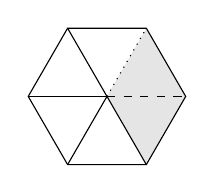
\begin{tikzpicture}
        \coordinate (O) at (0, 0);
        \coordinate (A) at ({cos(0)}, {sin(0)});
        \coordinate (B) at ({cos(60)}, {sin(60)});
        \coordinate (C) at ({cos(120)}, {sin(120)});
        \coordinate (D) at ({cos(180)}, {sin(180)});
        \coordinate (E) at ({cos(240)}, {sin(240)});
        \coordinate (F) at ({cos(300)}, {sin(300)});
        \fill[gray!20] (A) -- (B) -- (O) -- (F) -- cycle;
        \draw (A) -- (B) -- (C) -- (D) -- (E) -- (F) -- cycle;
        \draw[dashed] (O) -- (A); \draw[dotted] (O) -- (B); \draw (O) -- (C); \draw (O) -- (D); \draw (O) -- (E); \draw (O) -- (F);
    \end{tikzpicture}
    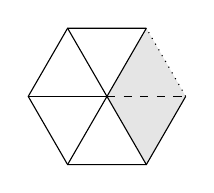
\begin{tikzpicture}
        \coordinate (O) at (0, 0);
        \coordinate (A) at ({cos(0)}, {sin(0)});
        \coordinate (B) at ({cos(60)}, {sin(60)});
        \coordinate (C) at ({cos(120)}, {sin(120)});
        \coordinate (D) at ({cos(180)}, {sin(180)});
        \coordinate (E) at ({cos(240)}, {sin(240)});
        \coordinate (F) at ({cos(300)}, {sin(300)});
        \fill[gray!20] (A) -- (B) -- (O) -- (F) -- cycle;
        \draw[dotted] (A) -- (B); \draw (B) -- (C) -- (D) -- (E) -- (F) -- (A);
        \draw[dashed] (O) -- (A); \draw (O) -- (B); \draw (O) -- (C); \draw (O) -- (D); \draw (O) -- (E); \draw (O) -- (F);
    \end{tikzpicture}
    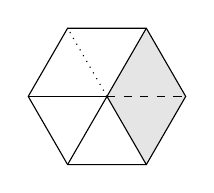
\begin{tikzpicture}
        \coordinate (O) at (0, 0);
        \coordinate (A) at ({cos(0)}, {sin(0)});
        \coordinate (B) at ({cos(60)}, {sin(60)});
        \coordinate (C) at ({cos(120)}, {sin(120)});
        \coordinate (D) at ({cos(180)}, {sin(180)});
        \coordinate (E) at ({cos(240)}, {sin(240)});
        \coordinate (F) at ({cos(300)}, {sin(300)});
        \fill[gray!20] (A) -- (B) -- (O) -- (F) -- cycle;
        \draw (A) -- (B) -- (C) -- (D) -- (E) -- (F) -- cycle;
        \draw[dashed] (O) -- (A); \draw (O) -- (B); \draw[dotted] (O) -- (C); \draw (O) -- (D); \draw (O) -- (E); \draw (O) -- (F);
    \end{tikzpicture}
    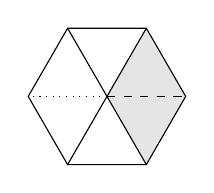
\begin{tikzpicture}
        \coordinate (O) at (0, 0);
        \coordinate (A) at ({cos(0)}, {sin(0)});
        \coordinate (B) at ({cos(60)}, {sin(60)});
        \coordinate (C) at ({cos(120)}, {sin(120)});
        \coordinate (D) at ({cos(180)}, {sin(180)});
        \coordinate (E) at ({cos(240)}, {sin(240)});
        \coordinate (F) at ({cos(300)}, {sin(300)});
        \fill[gray!20] (A) -- (B) -- (O) -- (F) -- cycle;
        \draw (A) -- (B) -- (C) -- (D) -- (E) -- (F) -- cycle;
        \draw[dashed] (O) -- (A); \draw (O) -- (B); \draw (O) -- (C); \draw[dotted] (O) -- (D); \draw (O) -- (E); \draw (O) -- (F);
    \end{tikzpicture}
    \caption{Examples and counterexamples for building a manifold-like $1$-patching of a $2$-dimensional manifold-like triangulation. (1) We have already added the edge patch along the dashed line and we add the edge patch along the dotted line. (2) The new edge patch already be a subset of the subtriangulation (3) An inadmissible choice because new edge patch has no overlap with current subtriangulation, though the next subtriangulation would be manifold-like (4) An inadmissible choice because new edge patch has no overlap with current subtriangulation and the next subtriangulation would not be manifold-like.}\label{figure:illustrationpatching}
\end{figure}

\begin{figure}
    \centering
    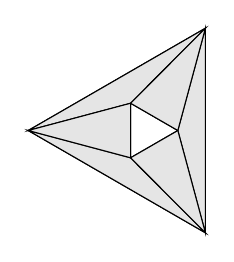
\begin{tikzpicture}[scale=0.5]
        \coordinate (O) at (0, 0);
        \coordinate (A) at ({0.8*cos(  0)}, {0.8*sin(  0)});
        \coordinate (B) at ({0.8*cos(120)}, {0.8*sin(120)});
        \coordinate (C) at ({0.8*cos(240)}, {0.8*sin(240)});
        \coordinate (X) at ({3.0*cos( 60)}, {3.0*sin( 60)});
        \coordinate (Y) at ({3.0*cos(180)}, {3.0*sin(180)});
        \coordinate (Z) at ({3.0*cos(300)}, {3.0*sin(300)});
        \draw (A) -- (B) -- (C) -- cycle; \draw (X) -- (Y) -- (Z) -- cycle;
        \draw[fill=gray!20] (X) -- (Y) -- (B) -- cycle;
        \draw[fill=gray!20] (Y) -- (Z) -- (C) -- cycle;
        \draw[fill=gray!20] (Z) -- (X) -- (A) -- cycle;
        \draw[fill=gray!20] (A) -- (X) -- (B) -- cycle;
        \draw[fill=gray!20] (B) -- (Y) -- (C) -- cycle;
        \draw[fill=gray!20] (C) -- (Z) -- (A) -- cycle;
    \end{tikzpicture}
    \begin{tikzpicture}[scale=0.5]
        \coordinate (O) at (0, 0);
        \coordinate (A) at ({3.0*cos(  0)}, {3.0*sin(  0)});
        \coordinate (B) at ({3.0*cos(120)}, {3.0*sin(120)});
        \coordinate (C) at ({3.0*cos(240)}, {3.0*sin(240)});
        \coordinate (X) at ({3.0*cos( 60)}, {3.0*sin( 60)});
        \coordinate (Y) at ({3.0*cos(180)}, {3.0*sin(180)});
        \coordinate (Z) at ({3.0*cos(300)}, {3.0*sin(300)});
        \draw (O) -- (A);
        \draw (O) -- (B);
        \draw (O) -- (C);
        \draw (O) -- (X);
        \draw (O) -- (Y);
        \draw (O) -- (Z);
        %
    \end{tikzpicture}
    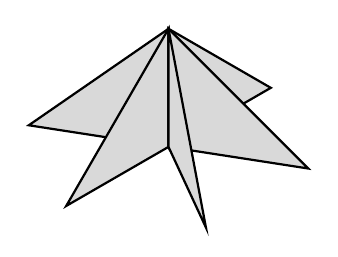
\begin{tikzpicture}[scale=0.5] 
        \tikzset{z={(90:1cm)}, y={(-30:1cm)}, x={(210:1cm)}}
        % \tikzset{z={(90:1cm)}, y={(-10:1cm)}, x={(250:1cm)}}

        \coordinate (O) at (0, 0);
        \coordinate (A) at ({3.0*cos(  0)}, {3.0*sin(  0)});
        \coordinate (B) at ({3.0*cos(120)}, {3.0*sin(120)});
        \coordinate (C) at ({3.0*cos(240)}, {3.0*sin(240)});
        \coordinate (X) at ({3.0*cos( 60)}, {3.0*sin( 60)});
        \coordinate (Y) at ({3.0*cos(180)}, {3.0*sin(180)});
        \coordinate (Z) at ({3.0*cos(300)}, {3.0*sin(300)});
        \coordinate (T) at ({0}, {0}, {3});

        \draw[thick, fill=gray!30] (O) -- (C) -- (T) -- cycle;
        \draw[thick, fill=gray!30] (O) -- (Y) -- (T) -- cycle;
        \draw[thick, fill=gray!30] (O) -- (Z) -- (T) -- cycle;
        \draw[thick, fill=gray!30] (O) -- (A) -- (T) -- cycle;
        \draw[thick, fill=gray!30] (O) -- (B) -- (T) -- cycle;
        \draw[thick, fill=gray!30] (O) -- (X) -- (T) -- cycle;
        
        
    \end{tikzpicture}

    \caption{Example of a connected $2$-dimensional manifold-like simplicial complex, which triangulates an annulus, that does neither admit a manifold-like $0$-patching nor manifold-like $1$-patching.}\label{figure:annuluscounterexample}
\end{figure}

% \color{red}
% \begin{proposition}
%     Suppose that $\calT$ is a connected $n$-dimensional simplicial complex. Then the following are equivalent:
%     \begin{itemize}
%      \item $\calT$ is manifold-like
%      \item $\calT$ has a manifold-like $0$-patching
%      % \item There exists $1 \leq k \leq n$ such that $\calT$ has a $k$-patching
%     \end{itemize}
% \end{proposition}
% \color{black}

% 4. Shellability 

We turn our attention to a different idea of how to incrementally construct a simplicial complex while maintaining well-behaved intermediate complexes. 
Given an $n$-dimensional simplicial complex $\calT$, a \emph{shelling} is an enumeration of the $n$-simplices $T_{0}, T_{1}, T_{2}, \dots \in \subsimplex_{n}(\calT)$ such that $( \calT(T_{0}) \cup \calT(T_{1}) \cup \dots \cup \calT(T_{m}) ) \cap \calT(T_{m+1})$ is a simplicial complex of dimension $n-1$. Notice that the last intersection is automatically a subcomplex of the boundary complex of the last simplex $T_{m}$, and is thus manifold like. 


% \begin{lemma}
%     If an $n$-dimensional simplicial complex $\calT$ has a shelling $T_{0}, T_{1}, T_{2}, \dots$, then it is manifold-like.
%     In particular, $\calT(T_{0}) \cup \calT(T_{1}) \cup \dots \cup \calT(T_{m})$ is manifold-like for every $m \geq 0$.
% \end{lemma}
% \begin{proof}    
% \end{proof}

We notion of shelling is taken from Ziegler's book~\cite{}

% TODO: Ziegler, Lemma 8.7: if a complex has a shelling, then this gives a shelling of the stars 

% 


\section{Constructive estimate of $p$-Poincar\'e constants}

% either proceeding simplex by simplex, matching along faces 
% or proceeding patch by patch, matching over intersections

\section{Constructive estimate of $p$-Poincar\'e--Friedrichs constants}
% Repeat for H(curl), H(div), and differential forms 

\section*{Acknowledgments}

\bibliographystyle{plain}
\bibliography{library}

\end{document}
